\clearpage
\section*{二、实验操作与原始数据}


\subsection*{1. 实验装置与原始记录}

实验使用 1 mA 电流计、FB711 型电压电流仪表校正仪、电阻箱、可调电阻、面包板和干电池。先测表头内阻，再完成 5 mA、5 V 单量程改装和校验，最后记录欧姆表的电阻—电流对应关系。

\begin{figure}[H]\centering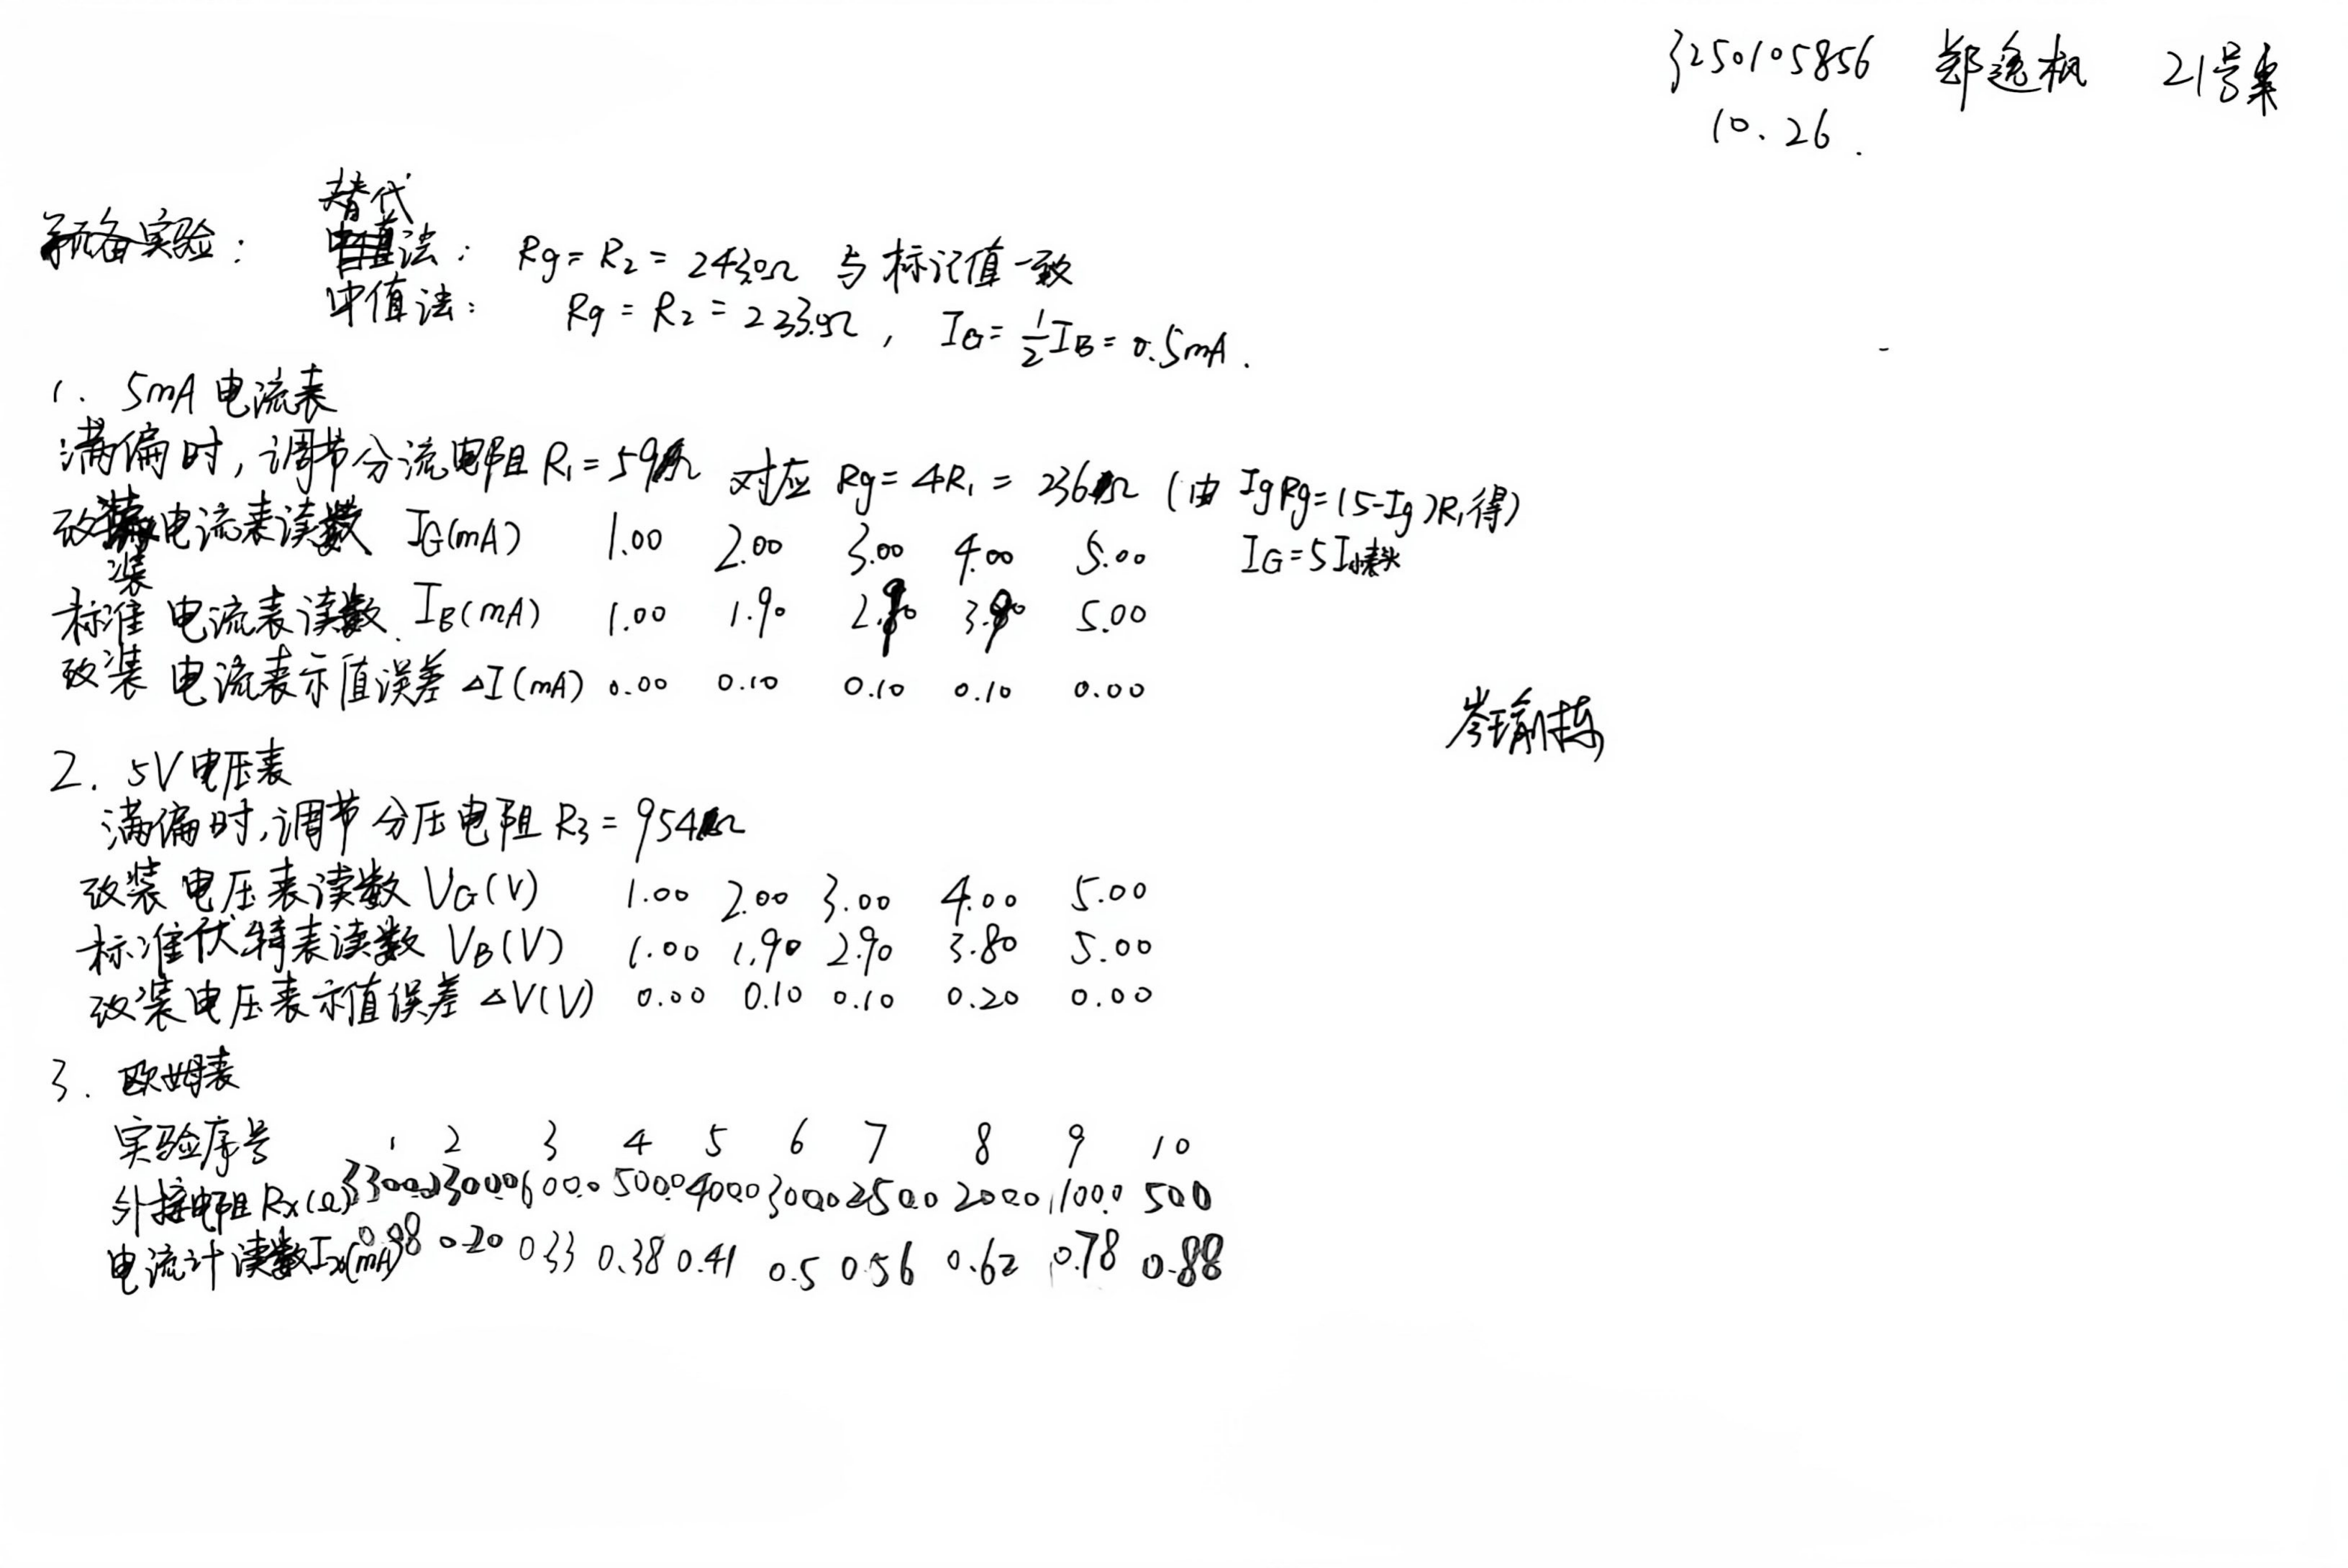
\includegraphics[width=.96\linewidth,height=10cm,keepaspectratio]{../assets/raw-data.png}\caption{原始测量记录（仅旋转阅读方向）}\end{figure}

\begin{figure}[H]\centering
\begin{minipage}[t]{.36\linewidth}\centering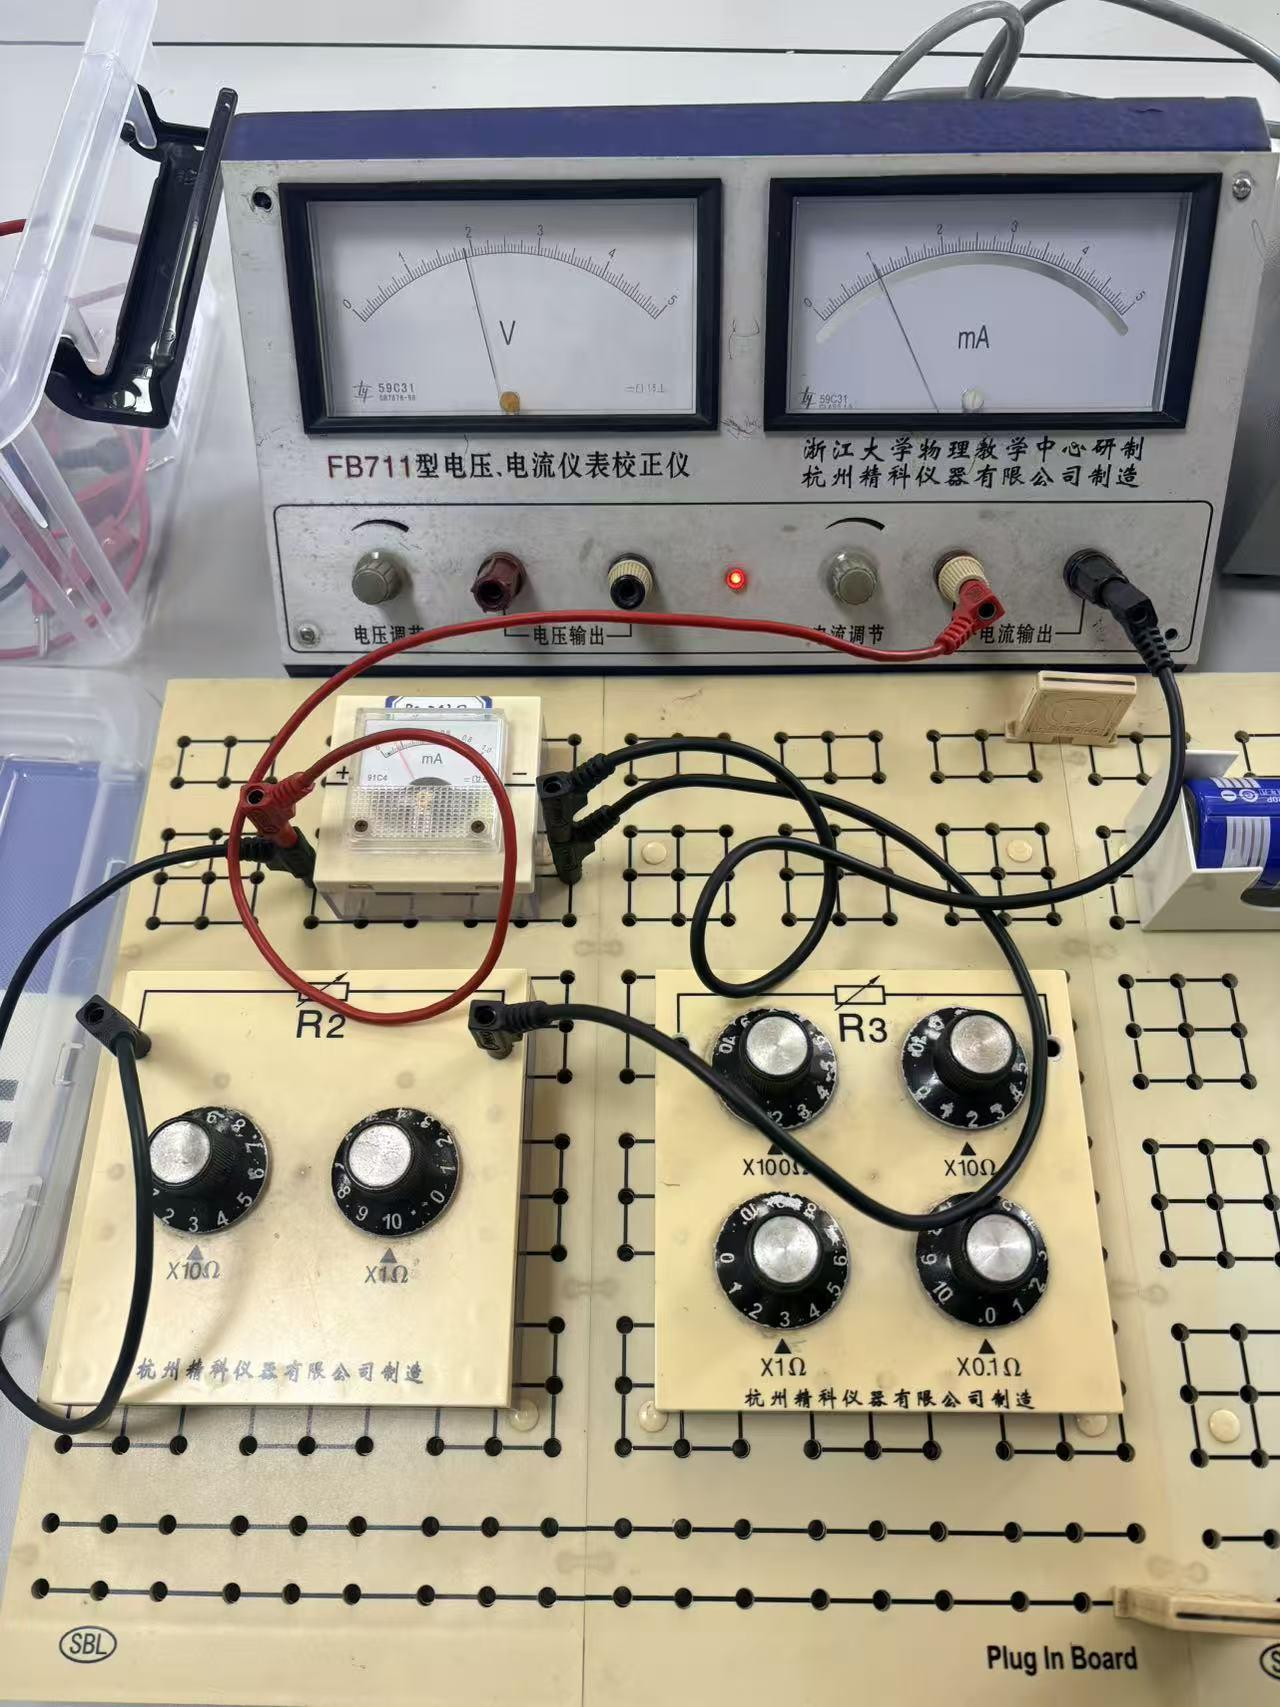
\includegraphics[height=4.5cm]{../assets/ammeter-setup.jpg}\caption{改装电流表的实验接线}\end{minipage}\hfill
\begin{minipage}[t]{.60\linewidth}\centering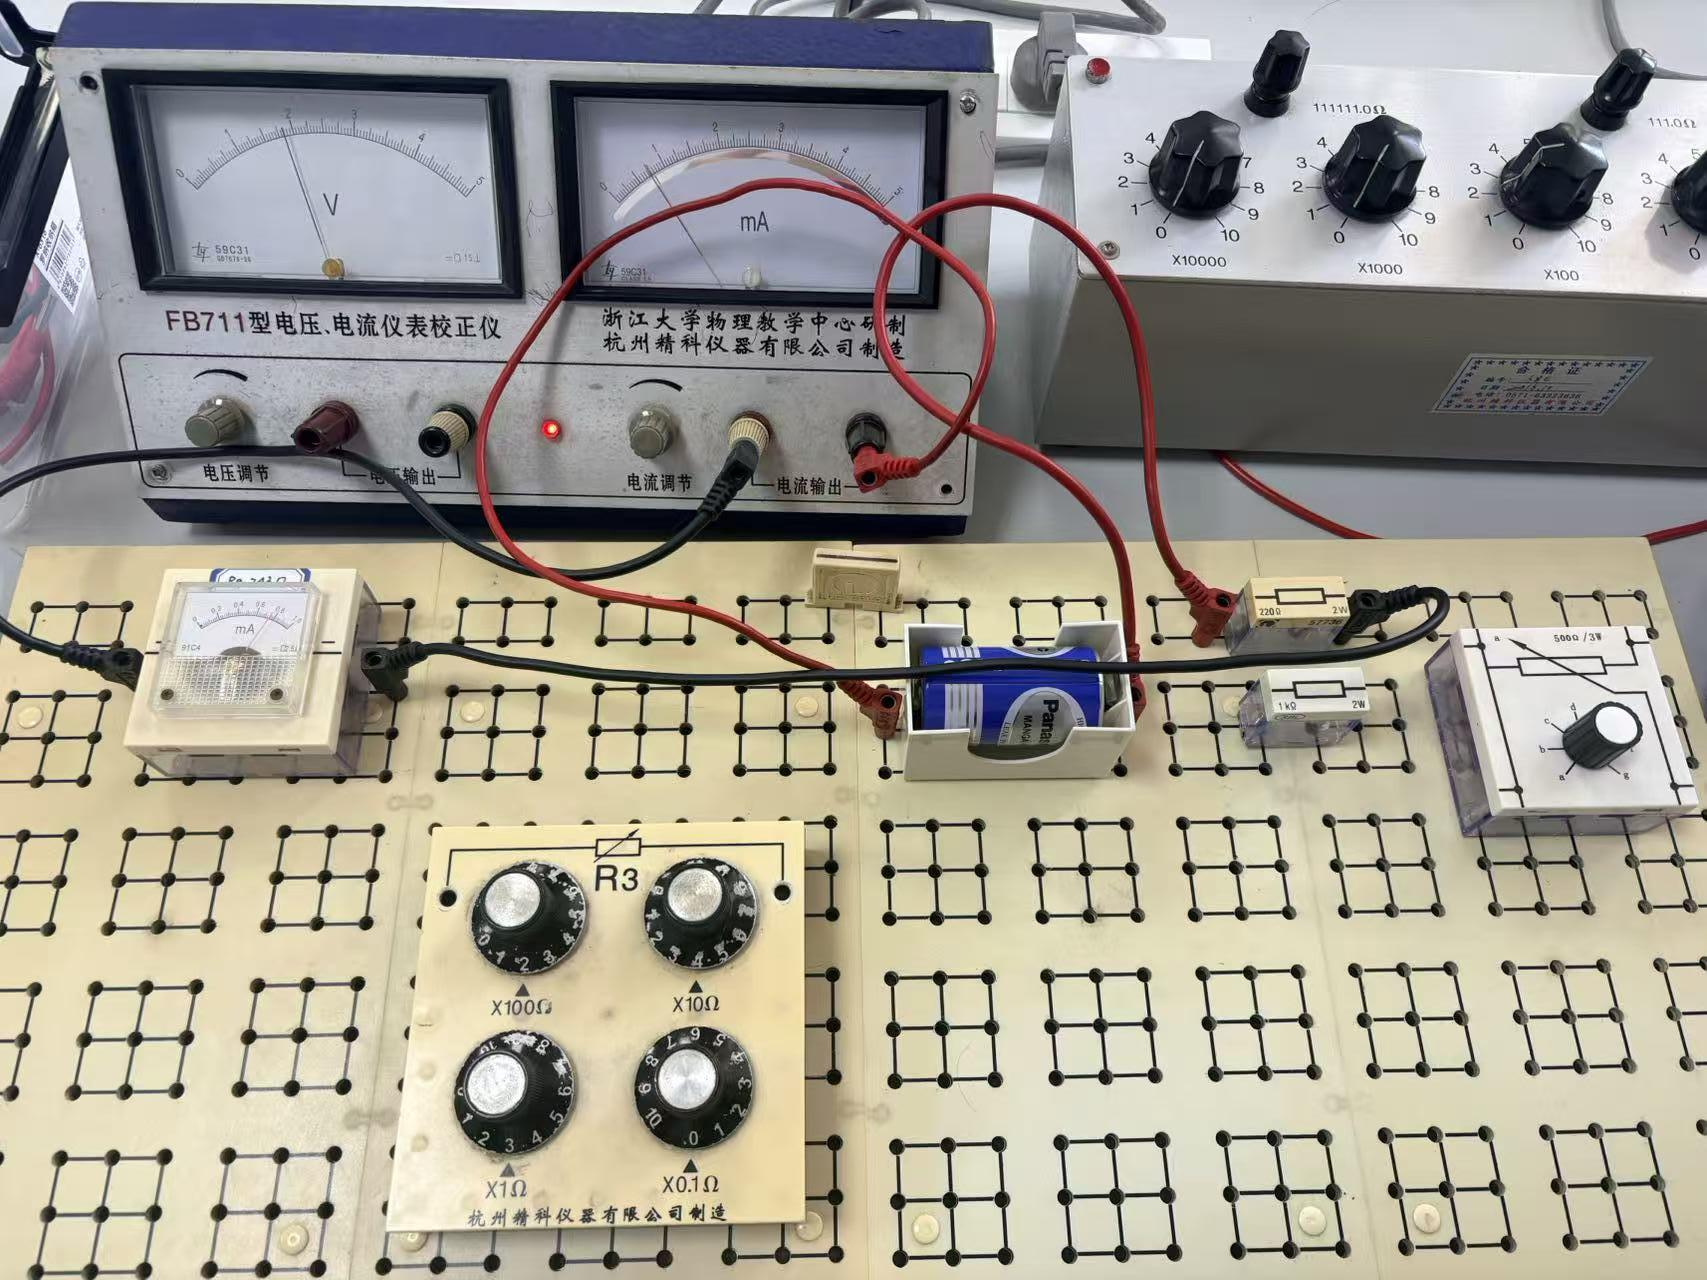
\includegraphics[height=4.5cm]{../assets/preliminary-setup.jpg}\caption{预备实验接线}\end{minipage}
\end{figure}
\newpage
\subsection*{2. 电流计内阻}

\begin{center}\small\setstretch{1.12}
\begin{tabularx}{\linewidth}{YYY}
\toprule
方法 & 内阻读数/Ω & 原始记录说明\\
\midrule
替代法 & 243 & 表头标记值 242 Ω\\
中值法 & 233.5 & 电流计半偏 0.5 mA\\
\bottomrule
\end{tabularx}\end{center}

\subsection*{3. 电流表校验}

满偏校准后分流电阻 $R_1=59\,\Omega$。

\begin{center}\small\setstretch{1.12}
\begin{tabularx}{\linewidth}{YYY}
\toprule
序号 & 改装表 $I_G$/mA & 标准表 $I_B$/mA\\
\midrule
1 & 1.00 & 1.00\\
2 & 2.00 & 1.90\\
3 & 3.00 & 2.90\\
4 & 4.00 & 3.90\\
5 & 5.00 & 5.00\\
\bottomrule
\end{tabularx}\end{center}

\subsection*{4. 电压表校验}

\begin{center}\small\setstretch{1.12}
\begin{tabularx}{\linewidth}{YYY}
\toprule
序号 & 改装表 $V_G$/V & 标准表 $V_B$/V\\
\midrule
1 & 1.00 & 1.00\\
2 & 2.00 & 1.90\\
3 & 3.00 & 2.90\\
4 & 4.00 & 3.90\\
5 & 5.00 & 5.00\\
\bottomrule
\end{tabularx}\end{center}

满偏校准后串联分压电阻 $R_3=954\,\Omega$。

\subsection*{5. 欧姆表读数}

电源电压为 1.5 V，保留并联分流电阻；短接时电流计示值为 1.00 mA。表中 $I_x$ 为电流计示值。

\begin{center}\small\setstretch{1.12}
\begin{tabularx}{\linewidth}{YYYYYY}
\toprule
序号 & $R_x$/Ω & $I_x$/mA & 序号 & $R_x$/Ω & $I_x$/mA\\
\midrule
1 & 3300.0 & 0.08 & 6 & 300.0 & 0.50\\
2 & 1300.0 & 0.20 & 7 & 250.0 & 0.56\\
3 & 600.0 & 0.33 & 8 & 200.0 & 0.62\\
4 & 500.0 & 0.38 & 9 & 100.0 & 0.78\\
5 & 400.0 & 0.41 & 10 & 50.0 & 0.88\\
\bottomrule
\end{tabularx}\end{center}


